\documentclass[a4paper, 12pt]{article}
\usepackage[left=2cm,right=2cm,top=2cm,bottom=2cm,bindingoffset=0cm]{geometry}
\usepackage[utf8]{inputenc}
\usepackage[english, russian]{babel}
\usepackage{amssymb, latexsym, amsmath}
\usepackage{indentfirst}
\usepackage{graphicx}
\usepackage{citehack}
\usepackage{tabularx}
\usepackage{listings}
\usepackage{pdfpages}
\usepackage{tikz}
\usepackage{pgfplots}

\lstloadlanguages{Python}
\lstset{extendedchars=false,
	breaklines=true,
	breakatwhitespace=true,
	keepspaces = true,
	tabsize=4
}

\begin{document}
\begin{titlepage}

\newpage

\begin{center}
Московский Авиационный Институт \\*
(национальный исследовательский университет) \\*

\vspace{2em}

Факультет прикладной математики и физики \\*
Кафедра вычислительной математики и программирования

\vspace{20em}

\Large \textbf{Лабораторная работа 2 \\*
по курсу <<Обработка естественых языков>>} \\*
II семестр

\end{center}

\vspace{15em}

\hspace{30em}\vbox{
	\hbox{Студент Данилычев И.\,А.}
	\hbox{Группа 8О-106М}
}

\vspace{\fill}

\begin{center}
Москва, 2016
\end{center}

\end{titlepage}

\newpage


\subsection*{Постановка задачи}
Построить график частотности терминов в зависимости от их позиции при сортировке по убыванию частоты. Подобрать параметры для формулы закона Ципфа
$$f(rank, s) = \dfrac{C}{{rank}^s}$$
для наилучшей аппроксимации.


\subsection*{Исходный код}
\lstinputlisting{../src/zipf.py}


\subsection*{Результат выполнения}
\begin{figure}[!htb]
	\centering
	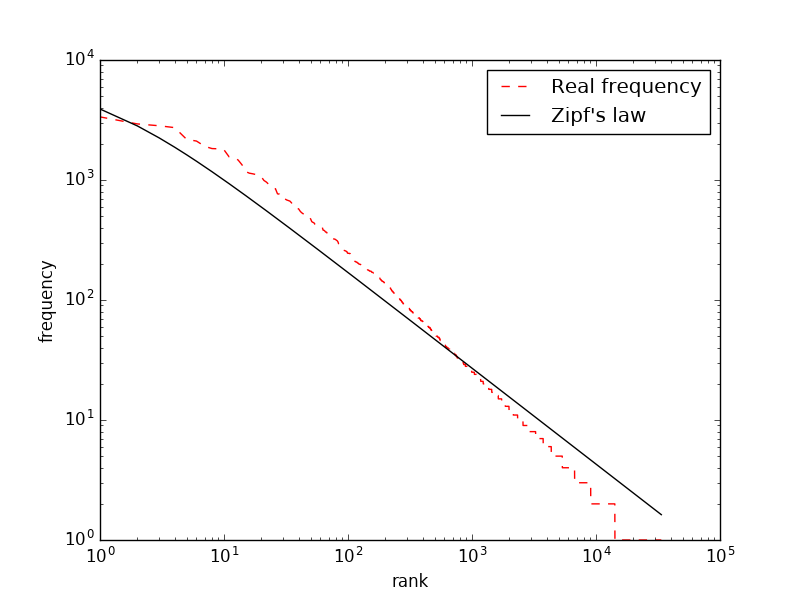
\includegraphics[scale=0.8]{zipf.png}
	\caption{Иллюстрация закона Ципфа для s = 0.8, C = 6800}
\end{figure}

\subsection*{Выводы}
Распределение частот терминов подчиняется закону, близкому к закону Ципфа, но на некоторых участках заметно расхождение этих двух кривых.
\end{document}

